\chapter{Implementación}

En este capitulo analizaremos la implementación realizada de los conceptos teóricos vistos hasta ahora y el uso practico de las tecnologías involucradas.

\medskip

El diseño de la aplicación esta basado en el patrón de software \emph{facade} con la idea de ofrecer una interfaz en C++ de tipo librería de alto nivel, reutilizable y fácil de usar, que permita realizar renderizados realistas sin tener que preocuparse de los detalles de bajo nivel relativos a OptiX y CUDA ni de todos los conceptos teóricos involucrados.

\medskip

Además sobre esta interfaz se ha construido un parser de escenas XML, para hacer aun mas sencillo el acto de configurar y crear escenas.

\clearpage

\section{Interfaz de programación}

\subsection{Estructura TCamera}

Este tipo de datos representa la cámara de la escena y encapsula todos los datos relativos a la cámara. Para construir un objeto de este tipo le pasamos la posición de la cámara, el posición del objetivo y el angulo de campo de visión.

\subsection{TSphereLight}

Esta estructura representa una luz esférica, tomando como parámetros la posición del centro de la esfera, su radio y una tripleta RGB representando su emisión de luz.

\subsection{TObjModel}

Es una estructura que representa un modelo 3D en formato .obj. Se construye pasándole la ruta del modelo. 

\subsection{Clase CPathtracer}

Este es el tipo de datos mas relevante de nuestra interfaz. Todos los datos relativos a la escena y al renderizado son finalmente encapsulados en un objeto de este tipo. Una vez configurado, es el responsable de cargar los programas de OptiX y construir el \emph{Context} de OptiX y controlar la ejecución del mismo.

\subsection{Uso de la interfaz de programación}

Para explicar el funcionamiento de la interfaz lo haremos mediante un sencillo ejemplo que contiene las clases y métodos principales de la interfaz.

\definecolor{orange}{rgb}{1.0,0.5,0.2}
\definecolor{purple}{rgb}{0.5,0.2,0.9}
\definecolor{blue}{rgb}{0.0,0.0,0.8}
\definecolor{green}{rgb}{0,0.7,0}
\definecolor{black}{rgb}{0.0,0.0,0.0}

\lstdefinestyle{customc}{
  belowcaptionskip=1\baselineskip,
  breaklines=true,
  frame=L,
  language=C,
  showstringspaces=false,
  basicstyle=\footnotesize\ttfamily,
  keywordstyle=\bfseries\color{green},
  commentstyle=\itshape\color{purple},
  identifierstyle=\color{blue},
  stringstyle=\color{orange},
}


\lstset{style=customc}

\begin{lstlisting}
CPathtracer pt;

pt.setRenderSize(width, height);
pt.setSqrtSamplesPerPixel(sqrtspp);
pt.setBlockSize(200u);
pt.setMaxDepth(7);


pt.setCamera(TCamera(optix::make_float3(8.0, 9.0, 1.0), 
		optix::make_float3(7.0, 9.0, 0.5), 60.0f));
pt.addObjModel(
		TObjModel("assets/dabrovic-sponza/sponza.obj"));
pt.addLight(TSphereLight(optix::make_float3(2.0f, 2.0f, 2.0f),
		optix::make_float3(0.0f, 5.0f, 0.0f), 1.0f));

pt.prepare();
pt.renderAllSamples();
pt.saveToTGA("render_sponza.tga");
\end{lstlisting}

Este ejemplo sirve para ilustrar el funcionamiento de la interfaz con el motor de renderizado.
Veamos el funcionamiento de este ejemplo:
En primer lugar creamos una instancia de la clase CPathtracer para seguidamente especificar las dimensiones, en pixeles, de la imagen que vamos a renderizar usando el metodo \emph{void setRenderSize(unsigned int width, unsigned int height)}. 

\medskip

Seguidamente usamos la instrucción \emph{pt.setSqrtSamplesPerPixel(sqrtspp} para especificar el numero de muestras por pixel. El valor que toma este método es la raíz cuadrada del numero de muestras. Lo hacemos de este modo para asegurarnos de que la división de cada pixel se hará en regiones uniformes dividiendo el pixel en \emph{sqrtspp} filas y \emph{sqrtspp} columnas.

\medskip

En la siguiente linea, especificamos un tamaño aproximado de los bloques en los que dividiremos la imagen. Entraremos en mas detalle sobre este comportamiento en las secciones siguientes pero de momento quedémonos con la idea de que la instrucción \emph{pt.setBlockSize(200u);} le dice al renderizador que debe dividir la imagen en bloques de aproximadamente 200x200 pixels. 

\medskip

A continuación especificamos la profundidad de recursión máxima. Este valor equivale al numero de veces que un rayo rebotara por la escena antes de ser terminado. Hay que calibrar bien este valor ya que un valor muy bajo produciría una iluminación pobre de la escena y un valor demasiado alto incrementaría el tiempo de ejecución innecesariamente.

\medskip

Seguidamente le pasamos al pathtracer un objeto de tipo TCamara inicializado con los valores de posición, objetivo y angulo de visión deseado. Solo puede haber una cámara activa a la vez por lo que la clase CPathtracer siempre usara la ultima que le especifiquemos.

\medskip

Los métodos \emph{addObjModel} y \emph{addLight} añaden modelos .obj y luces a la escena. A diferencia de la cámara, podemos llamar a estos métodos tantas veces como queramos para añadir luces y geometría a la escena.

\medskip

El método \emph{prepare} toma todos los datos de configuración que hemos especificado anteriormente y los compila en un \emph{Context} de OptiX para poder empezar el proceso de renderizado.

\medskip

Usamos la instrucción \emph{pt.renderAllSamples()} para efectuar un renderizado completo, de la imagen que tomara tantas muestras como hayamos especificado, y por ultimo guardamos el resultado en una fichero TGA. Por simplicidad en este ejemplo hemos usado el método \emph{renderAllSample} pero también existe la opción de renderizadar solo una muestra por pixel por llamada con el método \emph{void renderNextSample()}, este método sera útil cuando queramos dar un feedback visual del progreso del renderizado, calculando una muestra y pintando en pantalla el resultado cada vez.

\clearpage

\section{Renderizado por bloques}

Durante el proceso de implementación nos encontramos con una dificultad cuando se trataba de renderizar escenas con muchos polígonos: el sistema operativo impone un limite al tiempo de ejecución de una llamada a la GPU de unos pocos segundos. Si llamábamos a la ejecución de un Context de OptiX contra toda la imagen, es decir con tantos CUDA threads como pixels, el sistema operativo paraba la ejecución antes de que esta terminara.

\medskip

La solución que encontramos fue dividir la imagen en bloques de menor tamaño y lanzar una ejecución del Context para cada uno de estos bloques. Es como pintar varias imágenes de menor tamaño y luego juntarlas, con la diferencia de que mantenemos un buffer en la memoria del device, del tamaño de la imagen final, para no tener que hacer transacciones de memoria entre el host y el device ya que esto reduciría notablemente el rendimiento.

\clearpage

\section{Camara}

\subsection{Host}

En el host precalculamos los datos de la cámara que serán constantes durante la ejecución: los vetores de la base ortonormal del sistema de coordenadas de camara (front, left, up) y la relación (viewd) entre el vector front y el vector up en función del angulo de visión fov.

\begin{lstlisting}
TCamera::TCamera(optix::float3 aposition, optix::float3 atarget, float afov)
{
	is_ok = false;
	if(afov <= 0.0f || afov >= 179.0f) return;

	position = aposition;
	target = atarget;
	fov = afov;
	viewd = 0.0f;

	front = optix::normalize(target - position);
	left = optix::normalize(optix::cross(optix::make_float3(0.0f, 1.0f, 0.0f), front));
	up = optix::normalize(optix::cross(front, left));

	viewd = 1.0 / tanf( fov * 0.5f * DEG2RAD);
	is_ok = true;		
}
\end{lstlisting}

\clearpage

\subsection{Device}

En el device tenemos un programa encargado de generar los rayos primarios que se lanzaran desde la cámara, para ello se le pasan desde el host una serie de parametros necesarios para lanzar el rayo correcto.

\begin{lstlisting}
float2 offset = make_float2(offset_x, offset_y);
float2 startSample = make_float2(launch_index) + offset 
	+ make_float2(
	(float)(currentSample%sqrtspp) * (1.0f/(float)sqrtspp),
	(float)(currentSample/sqrtspp) * (1.0f/(float)sqrtspp)
);

float2 centerSample = make_float2(1.0f/float(2 * sqrtspp));
float2 d = (startSample + centerSample) / make_float2(screen_dim.x, screen_dim.y) * 2.f - 1.f;

d.x *= aspect_ratio;
float3 ray_origin = eye;
float3 ray_direction = normalize(d.x*U + d.y*V + W*viewd);
\end{lstlisting}

El offset son las coordenadas absolutas en espacio de imagen del pixel top-left del bloque que estamos pintando y el launch\_index es él indice del CUDA thread actual que se corresponde con las coordenadas relativas al bloque actual del pixel que estamos pintando. Usamos estas variables para calcular las coordenadas top-left del pixel estamos pintando, en coordenadas absolutas de la imagen entera.

\medskip

Para que el muestreo múltiple de cada pixel proporcione antialiasing es necesario dividir el pixel en regiones y lanzar el rayo a través de la región que se corresponde con la muestra actual. Para calcular las coordenadas de la región actual lo hacemos a partir del parámetro currentSample y de la raiz cuadrada del total de muestras (la variable sqrtspp).

\medskip

Efectuados estos cálculos tenemos las coordenadas top-left absolutas de la región de pixel. A estas coordenadas le sumamos el valor de media región de pixel para que el rayo salga por el centro de dicha región, en vez de por su esquina superior-izquierda.

\medskip

En la variable d normalizamos esas coordenadas para obtener las coordenadas de pantalla correctas en el intervalo $[-1, 1]$. Corregimos la relación de aspecto de la imagen y calculamos la dirección del rayo resultante.

\clearpage

\section{Muestreo de la BRDF}

Para el muestreo de la BRDF usamos el modelo propuesto en \cite{Lafortune1994} que hemos explicado en la sección \ref{muestreo_brdf}.
\medskip

En primer lugar decidimos aleatoriamente si muestrear la parte difusa o la parte especular de la BRDF. Para ello proponemos usar como probabilidades las medias de los valores RGB de las componentes difusa y especular: $p_{diff} =\frac{1}{3}( k_{dR} + k_{dG} + k_{dB})$ y $p_{spec} =\frac{1}{3}( k_{sR} + k_{sG} + k_{sB})$ 

\medskip

Generamos un un numero aleatorio $r$ en $[0,1]$ y si $r \leq p_{spec}$ muestreamos la parte especular, si $p_{spec} < r \leq p_{spec} + p_{diff}$ la parte difusa, en caso contrario el rayo es absorbido y terminamos la recursión del mismo.

\medskip

Esta forma de terminar la recursión se conoce como ruleta rusa y es una técnica de reducción de la variancia usado en integraciones por monte carlo. Para compensar esta terminación anticipada y la separación entre rayos difusos y especular dividiremos el resultado entre la probabilidad de que se lance ese rayo. Ya que se muestrea con mas probabilidad el evento mas probable esto servirá para dar mas peso a aquellas muestras menos probables.

\subsection{Muestreo de la parte difusa de la BRDF}
En el programa de closest hit, muestreamos la hemiesfiera centrada en el punto de intersección para tener una estimación de la luz incidente.

\begin{lstlisting}
	unsigned int seed = prd_radiance.seed;
	float r1 = rnd(seed);
	float r2 = rnd(seed);
	float3 p;
	cosine_sample_hemisphere(r1, r2, p);
	
	float3 u, v;
	createONB(ffnormal, u, v);
	float3 rd = normalize(u * p.x + v * p.y + ffnormal * p.z);
		
	PerRayData_radiance diffuse_refl_prd;
	diffuse_refl_prd.seed = seed;
	diffuse_refl_prd.depth = prd_radiance.depth + 1;
	diffuse_refl_prd.contribution *= Kd;
	diffuse_refl_prd.is_light = false;
	optix::Ray diffuse_refl_ray( hit, rd, radiance_ray_type, scene_epsilon );
	rtTrace(top_object, diffuse_refl_ray, diffuse_refl_prd);
	brdfLight = diffuse_refl_prd.result;
	color += brdfLight * Kd / prob_diff;
\end{lstlisting}

Basicamente lo que hace es, en el caso de que no hayamos llegado a la profundidad de recursión máxima, muestrear un punto en la hemiesfiera con densidad de coseno, generar una base ortonormal en función de la normal de la superficie y transformar el punto de la hemiesfera con esa base. Se traza un rayo recursivamente en la dirección obtenida y el color devuelto por ese rayo se multiplica por el color difuso de la superficie.

\medskip

Hay que hacer notar que en la instrucción \emph{color += brdfLight * Kd / prob\_diff;} no estamos multiplicando por el típico factor coseno de la normal y la luz. No lo hacemos porque al tomar la muestra con densidad coseno y dividir entre la densidad de probabilidad de esa muestra los factores coseno se anulan.
Siguiendo con ese razonamiento y teniendo en cuenta que la densidad coseno es $\frac{cos(l,n)}{\pi}$ deberíamos multiplicar el resultado por $\pi$ para ser coherentes con la teoría pero lo hemos quitado del cálculo porque hemos comprobado empíricamente que el resultado final es mas satisfactorio sin ese factor, que en caso de incluirlo en el cálculo generaba imágenes excesivamente iluminadas y quemadas.

\medskip

Usando tan solo esta función de iluminación ya es posible generar renderizados aunque al no muestrear las luces directamente tardaran mas en converger.
En las primeras fases de la implementación realizamos algunos renderizados con este closest hit program, y un closest hit program para las fuentes de luz que devolvía su emisión de luz.


\begin{figure}[h]
\centering
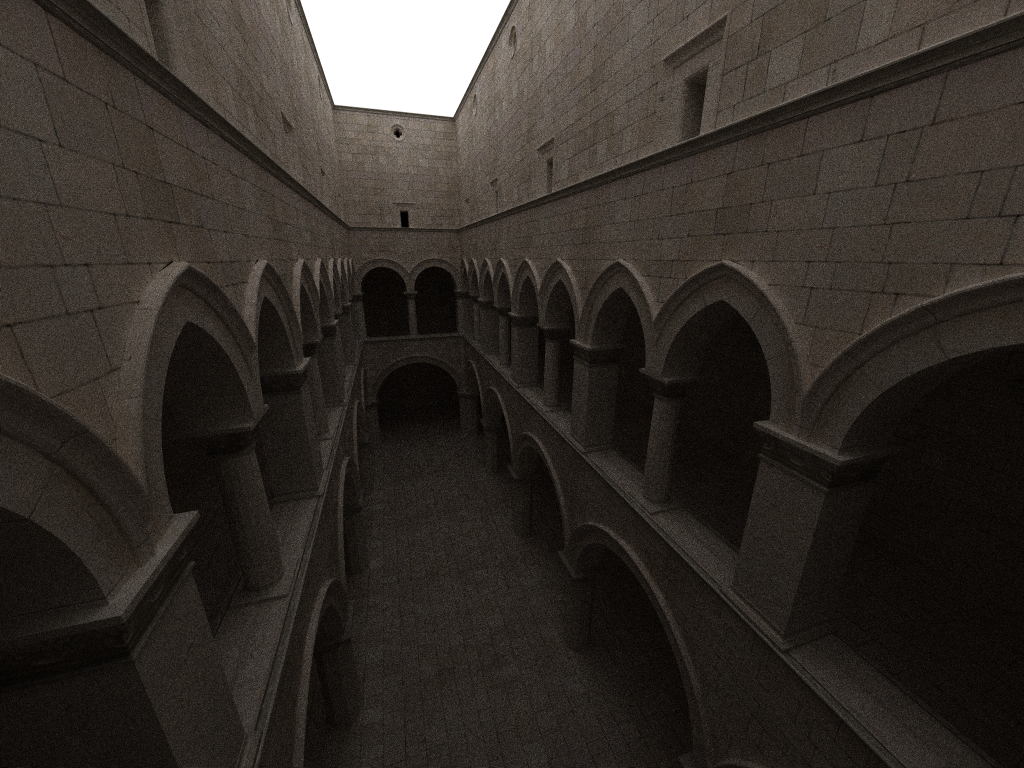
\includegraphics[width=5in]{dome1.png}
\caption{Muestreo de la brdf difusa}
\end{figure}

\clearpage

\subsection{Muestreo de la parte especular de la BRDF}

En el caso de la parte especular usamos como densidad de probabilidad una potencia de coseno de forma que el exponente sea mayor cuanto mas reflectante sea el material. Ese vector es posteriormente transformado con una base ortonormal orientada hacia la dirección de reflexion perfecta.

\begin{lstlisting}
	float3 eye = -ray.direction;
	float3 perfect_specular = normalize(2.0 * ffnormal * dot(ffnormal, eye) - eye);
	createONB(perfect_specular, u, v);
	p = sample_specular2(phong_exp, r1, r2);
	float3 rd = normalize(u * p.x + v * p.y + perfect_specular * p.z);
	if(dot(rd, ffnormal) > 0.0f){
		PerRayData_radiance specular_refl_prd;
		specular_refl_prd.seed = seed;
		specular_refl_prd.depth = prd_radiance.depth + 1;
		specular_refl_prd.contribution *= Ks;
		specular_refl_prd.is_light = false;
		optix::Ray specular_refl_ray( hit, rd, radiance_ray_type, scene_epsilon );
		rtTrace(top_object, specular_refl_ray, specular_refl_prd);
		brdfLight = specular_refl_prd.result;
				
		color += ( brdfLight * Ks * (phong_exp + 2) * dot(rd, ffnormal) ) / ( (phong_exp + 1) * prob_spec );
	}

\end{lstlisting}

\clearpage

\section{Muestreo de luces}

Una mejora importante que hemos implementado ha sido el muestreo directo de fuentes de luz. Muestrear las luces directamente provoca que el renderizado converja mas rápido al lanzar rayos hacia zonas de la escena que es mas probable que aporten luz al computo final.

\begin{lstlisting}

for(int i = 0; i < spherical_lights.size(); ++i){
	float3 light_dir = spherical_lights[i].center - hit;
	float dist2 = dot(light_dir, light_dir);
	float radius2 = spherical_lights[i].radius * spherical_lights[i].radius;
	if(dist2 - radius2 < scene_epsilon){
		continue;
	}
	unsigned int seed = prd_radiance.seed;
	float cos_theta_max = sqrtf(1 - radius2/dist2);
	float inv_pdf = 2.0f * PI * (1.0f - cos_theta_max);
	
	float r1 = rnd(seed);
	float r2 = rnd(seed);
	float cos_theta = 1 + r1 * (cos_theta_max - 1);
	float sin2theta = 1 - cos_theta * cos_theta;
	float sin_theta = sqrtf(sin2theta);
	float sin_phi = sinf(2 * PI * r2);
	float cos_phi = cosf(2 * PI * r2);
	float3 w = normalize(light_dir);
	float3 u, v;
	createONB(w, u, v);
	float3 dir = normalize( u * cos_phi * sin_theta + v * sin_phi * sin_theta + w * cos_theta );

	if(dot(dir, ffnormal) < 0) continue;
	PerRayData_shadow shadow_prd;
	shadow_prd.contribution = spherical_lights[i].emission;
	float delta = sqrtf(radius2 - sin2theta * dist2);
	Ray shadow_ray = Ray( hit, dir, shadow_ray_type, scene_epsilon, cos_theta * length(light_dir) - delta );
	rtTrace(top_object, shadow_ray, shadow_prd);
	color += inv_pdf * shadow_prd.contribution * dot(dir, ffnormal) * (Kd + Ks * powf(fmaxf(dot(dir, perfect_specular), 0.0f), phong_exp) );

}
\end{lstlisting}

Para cada luz esférica calculamos la distancia del punto que estamos evaluando al centro de la esfera y en caso de encontrarnos dentro de la misma la omitimos y continuamos con la siguiente.

\medskip


A continuación procedemos a generar una dirección dentro del angulo sólido subtendido por la esfera, tal como se ha explicado en la sección \ref{sample_solid}. Si dicha dirección forma un angulo superior a noventa grados con respecto a la normal la omitimos.

\begin{figure}[h]
\centering
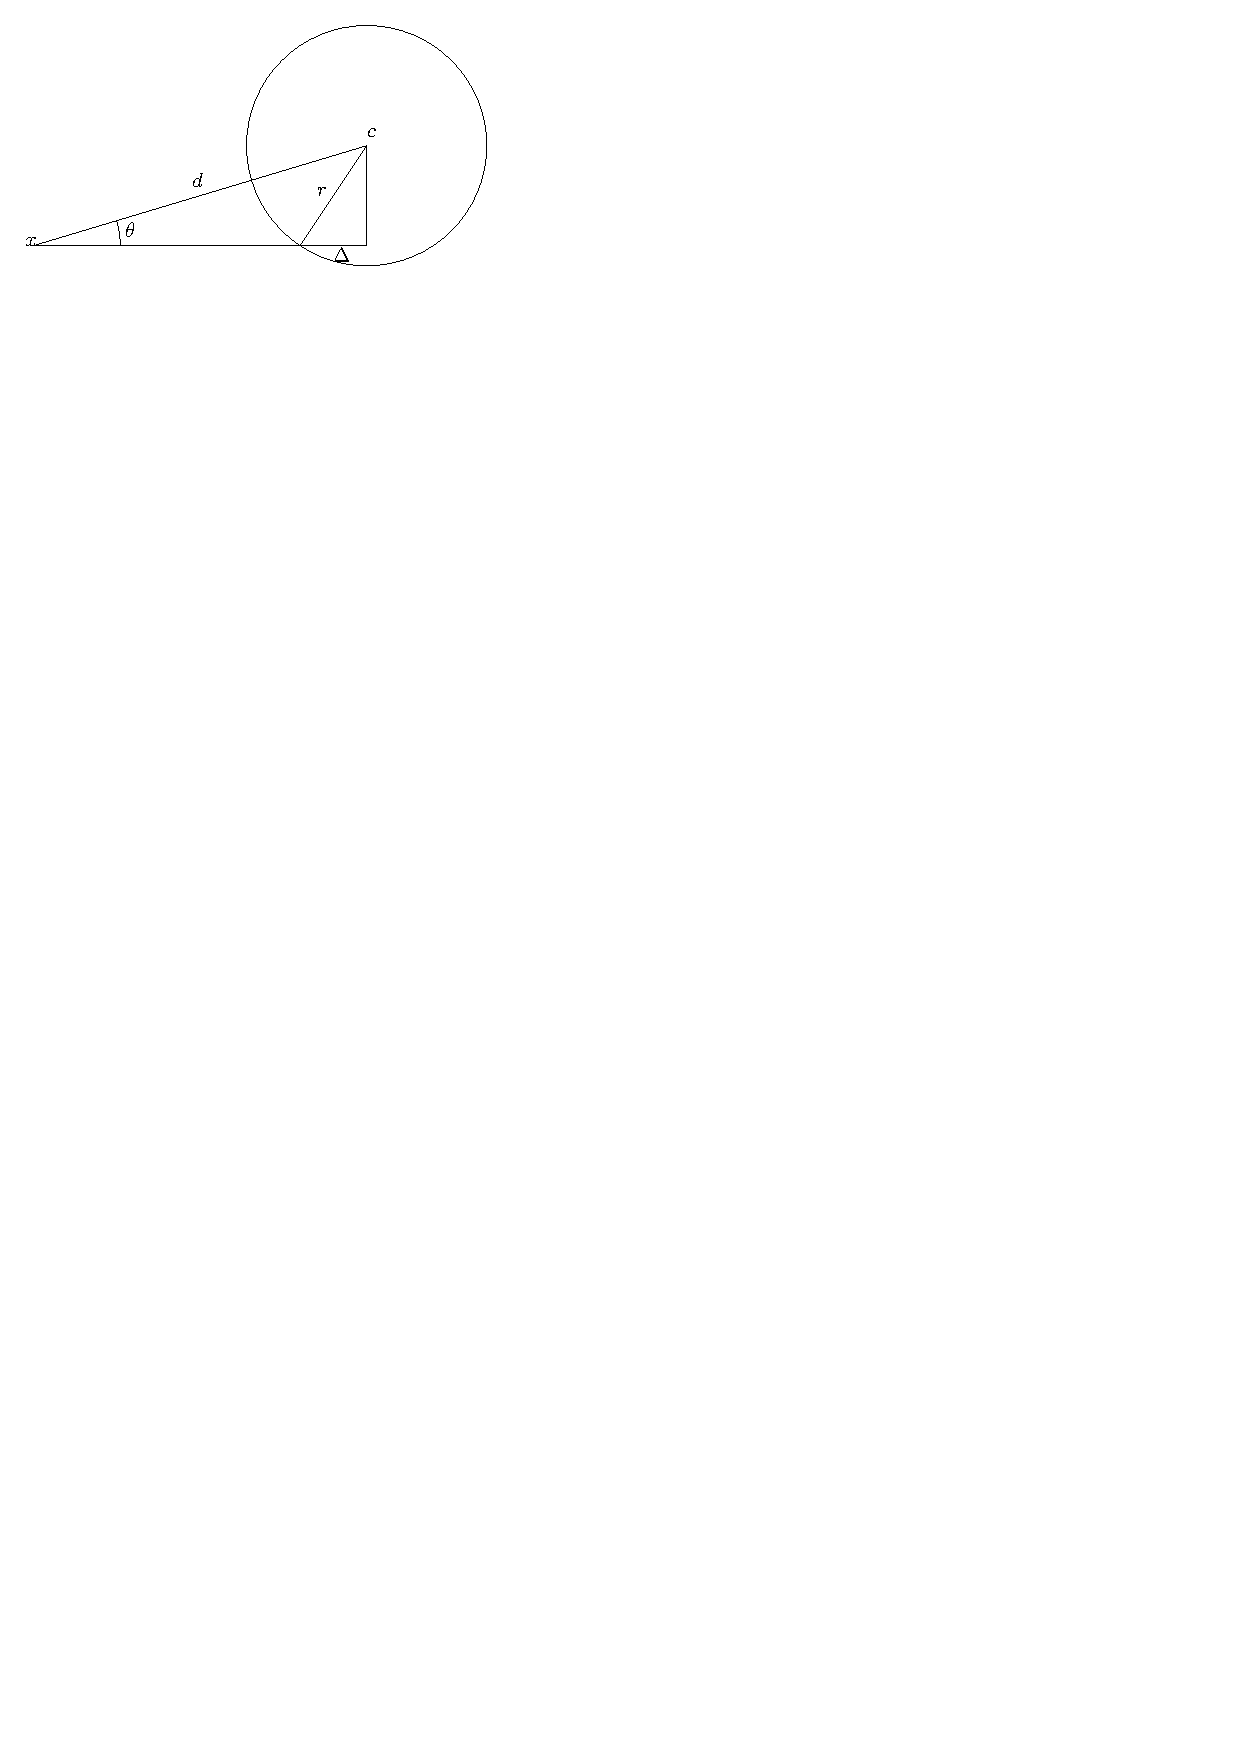
\includegraphics[scale=1.0]{sample_esfera.pdf}
\caption{  $\Delta $ al punto de intersección}
\end{figure}

La distancia a la que se encuentra el primer punto de intersección de la esfera con el rayo será $d_{intersect} = d \cos\theta - \Delta $. Este valor $\Delta = \sqrt{r^2 - (d\sin\theta)^2}$ lo calculamos en la instrucción \emph{float delta = sqrtf(radius2 - sin2theta * dist2);}. De este modo cuando creemos el rayo lo haremos con una distancia máxima que es la que nos interesa con tal de que no interseccione con objetos que estén dentro o detrás de la esfera. En las lineas 29 y 30 creamos y lanzamos el rayo. El valor \emph{shadow\_prd.contribution} será la emision de luz de la fuente que estamos muestreando o $0$ si ha interseccionado con algun objeto.

\medskip

Finalmente en la ultima linea calculamos la contribución de luz de la muestra evaluando la BRDF.




